%\documentclass[12pt]{IEEEtran}
\documentclass[12pt, a4paper]{article}
\usepackage{fancyhdr}

\begin{document}

\begin{titlepage}
	\begin{center}
	\huge{University of Pretoria\\
	Software Engineering 301 - COS 301}\\
	\line(1,0){400}\\
	\huge{\bfseries NavUp Software Requirements Specification}\\
	\line(1,0){200}\\
	Team Teal\\
	16 February 2017\\
	[3cm]
	\end{center}
	\begin{flushleft}
	\bfseries{Author(s):}
	\end{flushleft}
	\begin{flushleft}
	Tlaka Mankgwanyane	\hspace{10mm}{\textbf {u14351872}}\\
	Alberts Josef			\hspace{26mm}{\textbf{u14395283}}\\
	Oratile Motswagosele	\hspace{11mm}{\textbf{u15306195}}\\
	Carrim Muhammed		\hspace{14mm}{\textbf{u15019854}}\\
	Jackson Pearce			\hspace{22.5mm}{\textbf{u14044332}}\\
	Potgieter Linda		\hspace{21.6mm}{\textbf{u14070091}}\\
	Kanda Madimba			\hspace{19.5mm}{\textbf{u17289077}}\\
	\end{flushleft}
\end{titlepage}

\tableofcontents

\section{Introduction}
\subsection{Purpose} 
This is the system requirement specification (SRS) aims to refine and expand on the required capabilities of the NavUP system. This includes discussion of the individual low coupled subsystems, functional and quality requirements. This document is intended for the developers of the NavUP system as well as the clients who own the system. It will refine what is required of the system, what the main purpose of the system will be and what additional capabilities it will have. 
\subsection{Scope}
The system being designed will be able to guide a variety of users such as students, lecturers and visitors, through the University of Pretoria's (UP) various campuses. This system will be identified as the NavUP system, referencing the navigation it will provide to visitors of the UP campuses. The system will be able to route users between buildings and on a campus, as well as guiding them to the chosen lecture hall within the building. Push notifications will also be sent to the users through the application when he/she is near a venue where public events are currently or will in future occur. There will not be any push notifications sent if the users is not near the venue where these events will occur. The user will be able to create a profile which will unlock additional functionalities such as sharing locations with friends, saving frequently used places, and adding timetable integration. The application will also be able to notify a user about high traffic areas which the user may want to avoid in order to arrive earlier at his/her destination. The system aims to simplify all users' navigation through the various UP campuses, ensuring quicker navigation to destinations and avoidance of congested routes.     
\subsection{Definitions, Acronyms, and Abbreviation}
SRS - System Requirement Specification
UP - University of Pretoria
NavUp - The system being designed, acronym for Navigate(Nav) University of Pretoria (UP).
System - The NavUp system that is being designed.
Product/Application - NavUp system
Traffic - Areas in which there is a higher concentration of users which may affect arrival times.
Hot Spots - Areas in which there are wi-fi access for the users.
\subsection{Overview}
This document will provide more details abut the product (NavUp), including different interfaces, memory requirements, operations, as well as site adapt ion requirements. Functions, characteristics, constraints, and dependencies will be discussed. Lastly the document will elaborate on  the different requirements, including external interface and functional requirements.

\section{Overall Description}
	\subsection{Product Perspective}
		\subsubsection{System Interfaces}
		\subsubsection{User Interfaces}
		\subsubsection{Hardware Interfaces}
		\subsubsection{Software Interfaces}
		\subsubsection{Communication Interfaces}
		\subsubsection{Memory}
		\subsubsection{Operations}
		\subsubsection{Site Adaptation Requirements}
	\subsection{Product Functions}
	\subsection{User Characteristics}
	\subsection{Constraints}
	\subsection{Assumptions and Dependencies}

\section{Specific Requirements}
	\subsection{External Interface Requirements}
		\subsubsection{System Interfaces}
The software’s system interface includes Wi-Fi networking, the system uses Wi-Fi access points for detecting locations both indoors and outdoors. 
The system also uses the campus map database for locating routes and site information, that is, building names, addresses, etc. 
Based on the GPS and campus map database, the system provides route guidelines to lecture halls, libraries and cafeterias. 
Other geographical information/data is read from the GPS.\\\\
GPS satellite broadcasts signals which are received by the GPS receiver, the GPS receiver processes the navigation equations 
to determine the users current PVT, that is, position, velocity, and time. Therefore, based on the user input, the system will start by validating 
the given input and determine the user’s current position, then from the user’s position the system should display the route guidelines to the destination.\\

	\subsubsection{User Interfaces}
The NavUp system will presents/launches the login page/form for users to login. The users should login to access more features, 
such as getting directions, calendar, etc. If for any reason the user is not registered or authenticated, the user should be able to 
register by using the “Sign-up” option. So, provided that the user has successfully logged-in, the user can search for locations within 
the campus. However, there might be many routes leading to the destination, so the user should have an option to choose an optimal 
route out of many available routes. There are different types of users, of which are students, visitors and lecturers.\newline
The NavUp system should have a "settings" option so that users can customize the application according to their needs. 
The "settings" screen should display the user's options for application themes/colors, notification sounds, and fonts properties, etc.\\\\
Certain users have different roles, for example; students will most likely use the software to navigate to lecture halls and access academic calendars, 
but visitors will most likely use the software to navigate to offices and boardrooms or to find where their meetings are scheduled. 
Therefore, certain users will have different activities (based on their roles) available for use in the software (NavUp system).
 Therefore when the user inputs data, the system should communicate with the campus map database and the GPS to get locations and route guidelines.\\\\
The users, particularly students should have profiles/accounts where their recent searches and others activities can be stored. 
Therefore, the system should have an option for users to view their profiles, and that’s where they can see their search history or rather the most visited venue/location. \\

	\subsubsection{Hardware Interfaces}
Mobile phones and Wi-Fi routers are the primary hardware interfaces necessary for the NavUp system. The system should communicate
 with the Wi-Fi routers and make use of the Wi-Fi access points to determine routes and locations. The GPS will use broadcasted signals by 
the GPS satellites to get locations in real-time. \\

	\subsubsection{Software Interfaces}
The NavUp will run primarily on mobile phones (smart phones), therefore the application should be compatible across most, 
if not all ranges of mobile smart phones, that is, either the Android Operating System or the iOS. The NavUp system will make 
use of the Wi-Fi access points and GPS to determine the current location/position of the user both indoors and outdoors. The 
system will also use of web services to connect to the campus map database in order to determine routes and site information (building names, addresses, etc.). 
So, only the routes within the Hatfield campus are accessible and all the information is displayed in the system’s screen interface. 
The system will determine the current position of the user in real-time using the GPS. \\

	\subsubsection{Communication Interfaces}
{The system will frequently communicate with the map database and the GPS in order to determine 
locations and also get directions. The communication between the system and the campus map database is done through Wi-Fi access points and web services. 
The mobile Operating System handles all other internal communications for the systems’ performance and response time. 
The NavUp system should be more accurate as possible, that is to say, it shouldn’t necessarily detect the exact user’s location. 
However, it should be in range (within the radius of the user’s current location). When the system receives an input from the user, 
the system will communicate with the map database and the GPS to get locations and directions in real-time. The NavUp system should also allow 
for multiple users at the same time, this is to say, the system’s performance shouldn’t be proportional to the number of active users.} \\
	\subsection{Functional Requirements}
		\subsubsection{Types of Users}
			\begin{itemize}
				\item Students
				\begin{itemize}
					\item Undergrad
					\item Postgrad
				\end{itemize}
				
				\item Employees
				\begin{itemize}
					\item Lecturers
					\item Admin staff
					\item Internal constructors
				\end{itemize}
				
				\item Visitors
				\begin{itemize}
					\item Parents
					\item External constructors
					\item Prospective students
					\item Walk-ins
				\end{itemize}
				
				\item Administrators
				\begin{itemize}
					\item UP officials
					\item Student societies
					\item UP event management
				\end{itemize}
			\end{itemize}
		\subsubsection{Use Case Prioritization}
			\begin{itemize}
				\item Critical
					\begin{itemize}
						\item User identifies destination
						\item Application determines location
						\item A user must be able to see building names as he passes them
						\item A user must specify  the kind of access
						\item A user must be able to see the campus map without searching for a location
						\item Venues should be grouped into categories
							\begin{itemize}
							\item A user must select a destination from category without typing it out
							\end{itemize}
						\item A user must see all the routes o the venue
							\begin{itemize}
								\item Disabilities
								\item Avoiding pedestrian traffic congestion
							\end{itemize}
						\item The user must be able to see arrival time
					\end{itemize}
				\item important
					\begin{itemize}
						\item The UP admin must be able to update venues
						\item The app must sync with the university calendar
						\item The events manager must be able to update events on the app
						\item Venues must be associated with events going to take place there
 						\item The UP student societies must be able to update their calendars on the app
						\item Log all activities
						\item Log user preferences
					\end{itemize}
				\item Nice To Have
					\begin{itemize}
						\item Fitness track
						\item A brief history about campus building as the user passes them
						\item Reward system if certain milestones archived
						
					\end{itemize}

			\end{itemize}
		
		\subsection{Use Cases And Actor-Interaction}
			\begin{itemize}
				\item Figure1: Login
					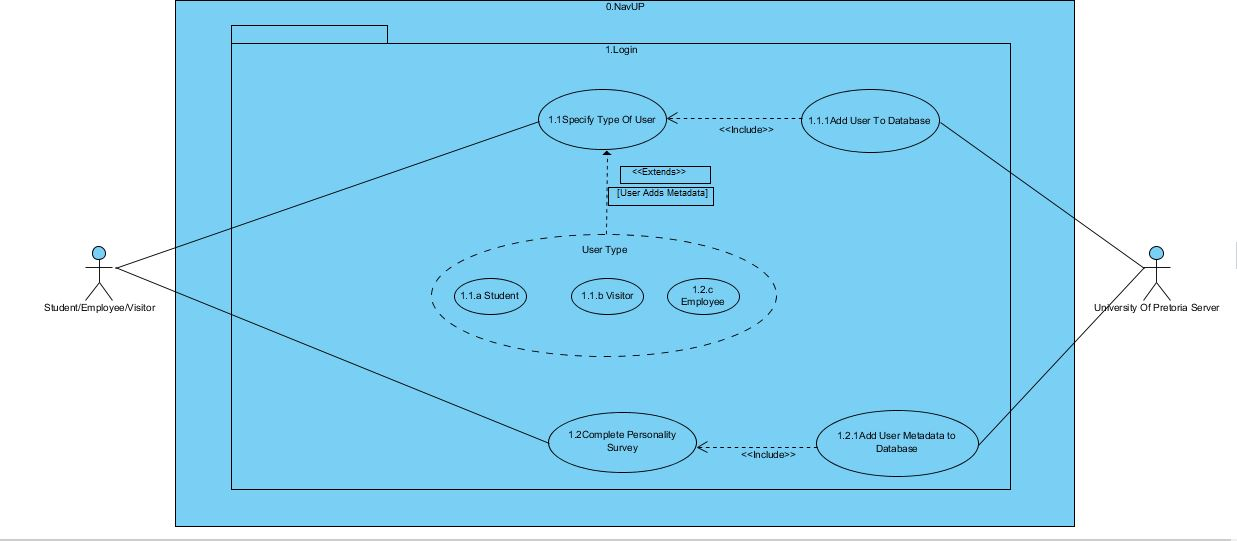
\includegraphics[width = 6cm, height = 10cm]{Login.JPG}
				\item Figure2: Select Destination
					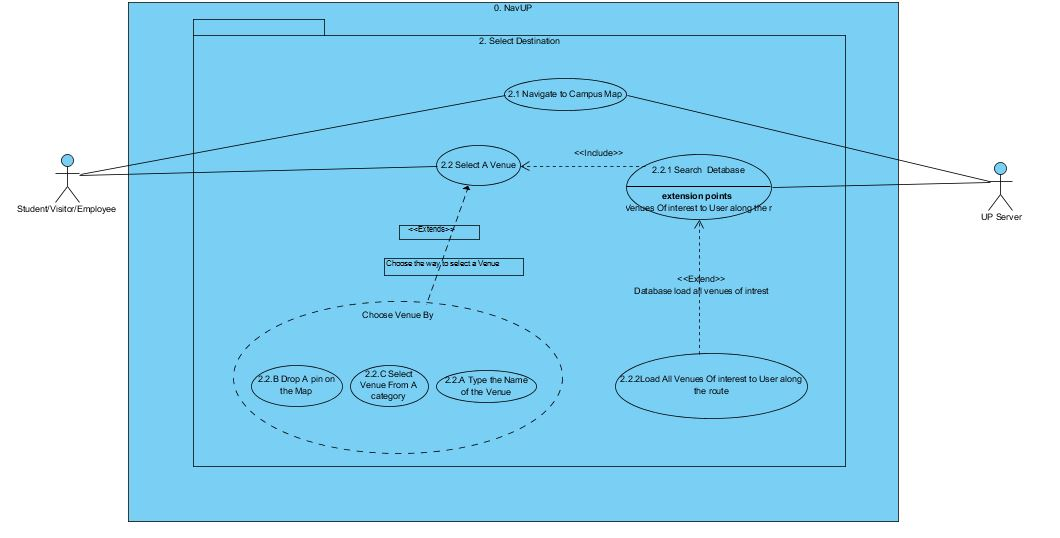
\includegraphics[width = 6cm, height = 10cm]{Select_Destination.JPG}
				\item Figure3: Route User
					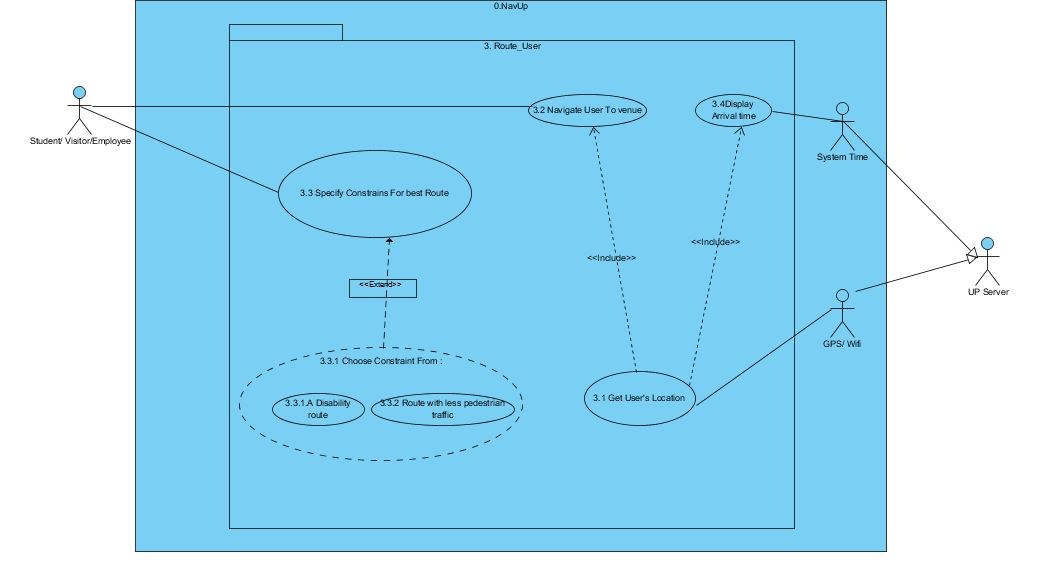
\includegraphics[width = 6cm, height = 10cm]{Route_User.JPG}
				\item Figure4: Login
					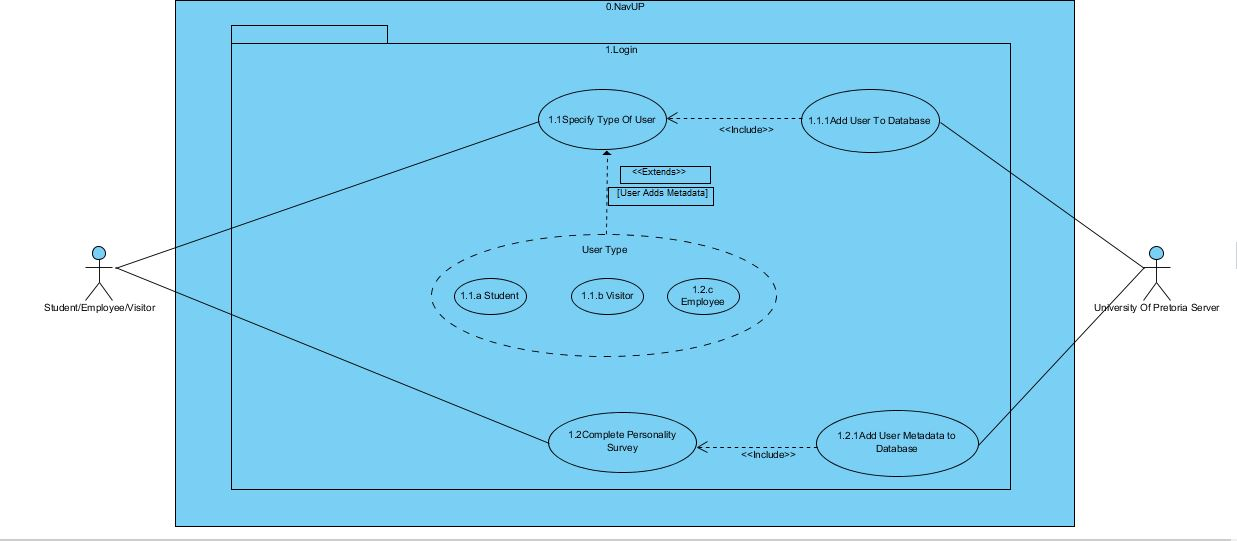
\includegraphics[width = 6cm, height = 10cm]{Login.JPG}
				\item Figure5: User fitness
					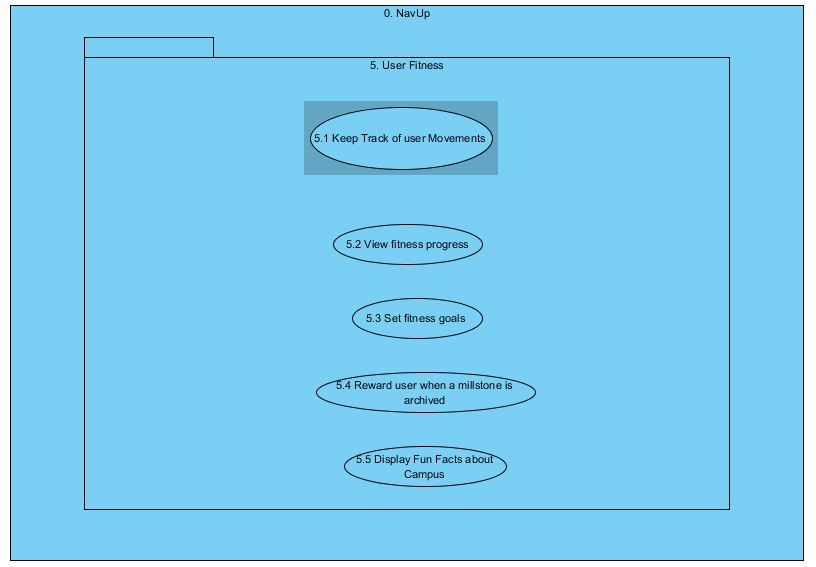
\includegraphics[width = 6cm, height = 10cm]{User_fitness.JPG}
			\end{itemize}
		
	\subsection{Performance Requirements}
		\subsubsection{Position Accuracy} The position of a device with NavUP activated should be accurately determined by the system - with no more than 15m of deviation from actual location of the device.
		\subsubsection{Time to Determine Position} It should take NavUP no longer than 45 seconds to determine the location of the device (with reasonable accuracy) once the application has been opened.
		\subsubsection{Immidiacy of Push Notifications} Relevant push notifications should be pushed to the user's device no further than 30m from the focus of said notification. For example, current events at the AULA should not be displayed if a user is further than 30m from the AULA, to prevent cluttering of the notification bar.
		\subsubsection{View/Location Updates} Updates of the user's current location as displayed on the device screen should take place at intervals of no more than 5 seconds.
		\subsubsection{User Login} Upon providing the system with correct credentials, the application must present the user with the navigation screen within 7 seconds. 
	\subsection{Design Constraints}
		\subsubsection{Operating System/Platform} The system must be accessible from both Android and iOS devices - natively.		
	\subsection{Software System Attributes}
		\subsubsection{Reliability} The system should never cease working completely unless the error is caused by external systems outside our control (operating system, web APIs, etc). Decoupling should be such that modules, such as information on landmarks, should still be accessible if navigation fails. Ideally an entire system uptime (per month) of 99.9\% must be reached.
		\subsubsection{Maintainability} The system's code must be well documented, both by means of in-code comments and external documentation, to aid in maintaining the system.
		\subsubsection{Security \& Privacy} NavUP will allow user profiles to be created and personal information to be stored, no unauthorized users should have access to another user's information. Only administrators or the owner of the profile in question should have access to a profile's data.
		\subsubsection{Portability} The system must be available on both Android and iOS devices.
		\subsubsection{Scalability} It must be possible to scale the system backend in the event of an increase of users. Scaling must be possible both horizontally or vertically.
		\subsubsection{Response time} Following user interaction, the system may not delay more than 2 seconds before providing the user with feedback.
		\subsubsection{Usability} NavUP's core functions (navigation, news updates, suggestions) must be easy to understand and use. They must not take the average user more than a minute, each, to access and understand. 
\end{document}
